\documentclass[12pt,a4paper]{article}
\usepackage[utf8]{inputenc}
\usepackage[T1]{fontenc}
\usepackage{graphicx}
\usepackage{hyperref}
\usepackage{geometry}
\usepackage{setspace}
\usepackage{xcolor}
\usepackage{titlesec}
\usepackage{enumitem}
\usepackage{fancyhdr}
\usepackage{listings}
\usepackage{tikz}
\usepackage{tikz-3dplot}
\usetikzlibrary{shapes,arrows,positioning,fit,backgrounds,calc,shadows}
\usepackage{tabularx}
\usepackage{booktabs}
\usepackage{float}

% Layout
\geometry{margin=1in}
\setstretch{1.15}
\pagestyle{fancy}
\fancyhf{}
\rhead{\textbf{Federated ICS Engine – Architecture \& Design}}
\lhead{System Architecture Document}
\rfoot{\thepage}

% Section formatting
\titleformat{\section}{\large\bfseries\color{blue!60!black}}{\thesection.}{1em}{}
\titleformat{\subsection}{\bfseries\color{black}}{\thesubsection}{1em}{}
\titleformat{\subsubsection}{\bfseries\color{gray}}{\thesubsubsection}{1em}{}

% Code listing style
\lstset{
    basicstyle=\ttfamily\small,
    breaklines=true,
    frame=single,
    backgroundcolor=\color{gray!10}
}

\begin{document}

\begin{center}
    \vspace*{0.5cm}
    {\Huge \textbf{Federated ICS Threat Correlation Engine}}\\[0.4cm]
    {\LARGE System Architecture \& Design Document}\\[0.3cm]
    {\large Version 1.0}\\[0.2cm]
    \textit{Industrial Control Systems Security Team}\\[0.1cm]
    \textbf{Date:} \today\\
    \vspace{0.5cm}
\end{center}

\tableofcontents
\newpage

\section{Executive Summary}

This document provides a comprehensive architectural and design specification for the Federated ICS Threat Correlation Engine.
The system is designed to provide real-time threat detection, attack prediction, and privacy-preserving collaborative defense for industrial control systems across multiple facilities.

\subsection{Document Purpose}

This architecture document serves as:
\begin{itemize}[leftmargin=1cm,itemsep=0pt]
    \item Technical blueprint for system implementation
    \item Reference for development teams
    \item Guide for deployment and operations
    \item Foundation for security audits and compliance
\end{itemize}

\subsection{Key Architectural Goals}

\begin{enumerate}[leftmargin=1cm,itemsep=0pt]
    \item \textbf{Real-Time Detection:} Detect threats within 30 seconds
    \item \textbf{High Accuracy:} >95\% detection accuracy, <5\% false positives
    \item \textbf{Privacy-Preserving:} Mathematical privacy guarantees (ε=2.0, δ=10⁻⁵)
    \item \textbf{Scalability:} Support 10-1000+ facilities
    \item \textbf{Resilience:} Byzantine-robust against malicious participants
    \item \textbf{Modularity:} Loosely coupled components for maintainability
\end{enumerate}

\subsection{Design Principles}

\textbf{1. Defense in Depth:} Multiple layers of security (network, application, data)

\textbf{2. Privacy by Design:} Data never leaves facility, privacy at every layer

\textbf{3. Fail-Safe:} System degrades gracefully under attack or failure

\textbf{4. Observable:} Comprehensive monitoring and logging

\textbf{5. Scalable:} Horizontal scaling for all components

\textbf{6. Standards-Based:} Use industry-standard protocols and frameworks

\section{System Overview}

\subsection{High-Level Architecture}

The system consists of six primary layers working together to provide comprehensive threat detection and collaborative defense.

\begin{figure}[H]
\centering
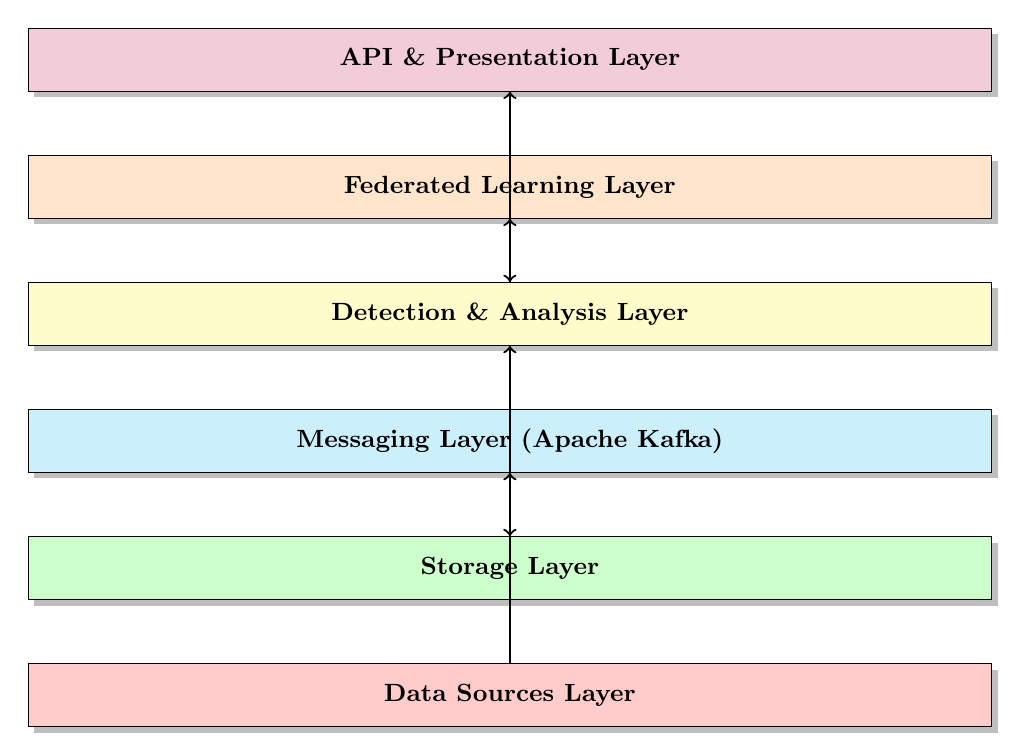
\begin{tikzpicture}[
    node distance=0.8cm,
    layer/.style={rectangle, draw, fill=blue!20, text width=12cm, align=center, minimum height=0.8cm, font=\bfseries\small, drop shadow},
    component/.style={rectangle, draw, fill=green!15, text width=2.5cm, align=center, minimum height=0.7cm, rounded corners, font=\scriptsize}
]

% Layers from top to bottom
\node[layer, fill=purple!20] (api) {API \& Presentation Layer};
\node[layer, below=of api, fill=orange!20] (fl) {Federated Learning Layer};
\node[layer, below=of fl, fill=yellow!20] (detection) {Detection \& Analysis Layer};
\node[layer, below=of detection, fill=cyan!20] (messaging) {Messaging Layer (Apache Kafka)};
\node[layer, below=of messaging, fill=green!20] (storage) {Storage Layer};
\node[layer, below=of storage, fill=red!20] (sources) {Data Sources Layer};

% Arrows showing data flow
\draw[->, thick] (sources) -- (messaging);
\draw[->, thick] (messaging) -- (detection);
\draw[->, thick] (detection) -- (storage);
\draw[->, thick] (detection) -- (fl);
\draw[->, thick] (fl) -- (api);
\draw[->, thick] (api) -- (detection);

\end{tikzpicture}
\caption{High-Level System Architecture - Six-Layer Design}
\end{figure}

\subsection{Architecture Layers}

\subsubsection{Layer 1: Data Sources Layer}

Ingests data from industrial control systems:
\begin{itemize}[leftmargin=1cm,itemsep=0pt]
    \item Industrial protocols (Modbus, DNP3, OPC-UA, S7)
    \item Network traffic (pcap, NetFlow)
    \item SCADA logs and events
    \item Physical sensor readings
\end{itemize}

\subsubsection{Layer 2: Storage Layer}

Polyglot persistence for different data types:
\begin{itemize}[leftmargin=1cm,itemsep=0pt]
    \item \textbf{Apache IoTDB:} Time-series sensor data
    \item \textbf{PostgreSQL:} Alerts, incidents, metadata
    \item \textbf{MongoDB:} Logs, protocol messages
    \item \textbf{Neo4j:} Attack graphs, MITRE ATT\&CK relationships
\end{itemize}

\subsubsection{Layer 3: Messaging Layer}

Apache Kafka message bus:
\begin{itemize}[leftmargin=1cm,itemsep=0pt]
    \item Decouples producers and consumers
    \item High-throughput data streaming
    \item Message persistence and replay
    \item Topic-based routing
\end{itemize}

\subsubsection{Layer 4: Detection \& Analysis Layer}

Core threat detection components:
\begin{itemize}[leftmargin=1cm,itemsep=0pt]
    \item LSTM Autoencoder (behavioral anomalies)
    \item Isolation Forest (point anomalies)
    \item Physics Rules Engine (process violations)
    \item Protocol Anomaly Detection
    \item Correlation Engine (multi-source fusion)
    \item Attack Prediction GNN
\end{itemize}

\subsubsection{Layer 5: Federated Learning Layer}

Collaborative learning infrastructure:
\begin{itemize}[leftmargin=1cm,itemsep=0pt]
    \item FL Client (local training)
    \item FL Server (aggregation)
    \item Privacy Engine (differential privacy)
    \item Secure Aggregation
    \item Byzantine-Robust Aggregation
\end{itemize}

\subsubsection{Layer 6: API \& Presentation Layer}

External interfaces:
\begin{itemize}[leftmargin=1cm,itemsep=0pt]
    \item REST API (CRUD operations)
    \item GraphQL API (flexible queries)
    \item WebSocket (real-time updates)
    \item Web Dashboard (React)
    \item Mobile App (future)
\end{itemize}

\section{Detailed Component Architecture}

\subsection{Data Sources Layer Components}

\begin{figure}[H]
\centering
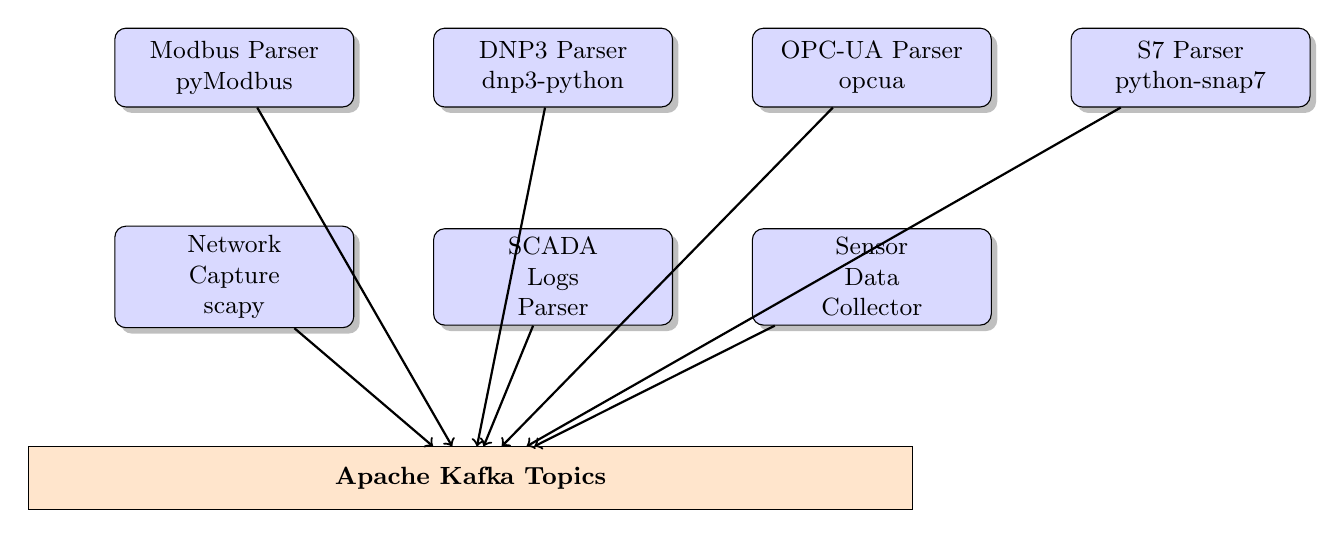
\begin{tikzpicture}[
    node distance=1cm,
    component/.style={rectangle, draw, fill=blue!15, text width=2.8cm, align=center, minimum height=1cm, rounded corners, font=\small, drop shadow},
    kafka/.style={rectangle, draw, fill=orange!20, text width=11cm, align=center, minimum height=0.8cm, font=\bfseries\small}
]

\node[component] (modbus) {Modbus Parser\\pyModbus};
\node[component, right=of modbus] (dnp3) {DNP3 Parser\\dnp3-python};
\node[component, right=of dnp3] (opcua) {OPC-UA Parser\\opcua};
\node[component, right=of opcua] (s7) {S7 Parser\\python-snap7};

\node[component, below=1.5cm of modbus] (pcap) {Network\\Capture\\scapy};
\node[component, right=of pcap] (scada) {SCADA\\Logs\\Parser};
\node[component, right=of scada] (sensors) {Sensor\\Data\\Collector};

\node[kafka, below=1.5cm of pcap, xshift=3cm] (kafka) {Apache Kafka Topics};

\draw[->, thick] (modbus) -- (kafka);
\draw[->, thick] (dnp3) -- (kafka);
\draw[->, thick] (opcua) -- (kafka);
\draw[->, thick] (s7) -- (kafka);
\draw[->, thick] (pcap) -- (kafka);
\draw[->, thick] (scada) -- (kafka);
\draw[->, thick] (sensors) -- (kafka);

\end{tikzpicture}
\caption{Data Sources Layer - Protocol Parsers and Collectors}
\end{figure}

\subsubsection{Protocol Parser: Modbus}

\textbf{Purpose:} Parse Modbus TCP/RTU protocol messages

\textbf{Responsibilities:}
\begin{itemize}[leftmargin=1cm,itemsep=0pt]
    \item Decode Modbus frames
    \item Extract function codes, addresses, values
    \item Detect malformed messages
    \item Publish to Kafka topic: \texttt{protocol.modbus}
\end{itemize}

\textbf{Technology:} Python 3.9+, pyModbus library

\textbf{Inputs:} TCP packets (port 502) or serial data

\textbf{Outputs:} JSON messages to Kafka
\begin{lstlisting}[language=json]
{
  "timestamp": "2025-10-13T14:23:45Z",
  "source_ip": "192.168.1.10",
  "function_code": 3,
  "address": 1000,
  "value": 42,
  "unit_id": 1
}
\end{lstlisting}

\textbf{Configuration:}
\begin{lstlisting}[language=yaml]
modbus:
  interface: eth0
  port: 502
  timeout: 5
  kafka_topic: protocol.modbus
  batch_size: 100
\end{lstlisting}

\subsubsection{Protocol Parser: DNP3}

\textbf{Purpose:} Parse DNP3 protocol (common in utilities)

\textbf{Responsibilities:}
\begin{itemize}[leftmargin=1cm,itemsep=0pt]
    \item Decode DNP3 frames
    \item Extract object variations, points
    \item Handle fragmentation
    \item Publish to Kafka topic: \texttt{protocol.dnp3}
\end{itemize}

\textbf{Technology:} Python 3.9+, dnp3-python

\textbf{Key Features:}
\begin{itemize}[leftmargin=1cm,itemsep=0pt]
    \item Master/Outstation communication
    \item Unsolicited response handling
    \item Integrity polls and event scans
\end{itemize}

\subsubsection{Protocol Parser: OPC-UA}

\textbf{Purpose:} Parse OPC-UA protocol (modern industrial standard)

\textbf{Responsibilities:}
\begin{itemize}[leftmargin=1cm,itemsep=0pt]
    \item Connect to OPC-UA servers
    \item Subscribe to data changes
    \item Monitor method calls
    \item Publish to Kafka topic: \texttt{protocol.opcua}
\end{itemize}

\textbf{Technology:} Python 3.9+, opcua library

\textbf{Security Features:}
\begin{itemize}[leftmargin=1cm,itemsep=0pt]
    \item Certificate-based authentication
    \item Encrypted communication
    \item User access control monitoring
\end{itemize}

\subsubsection{Network Capture Component}

\textbf{Purpose:} Capture and analyze network traffic

\textbf{Responsibilities:}
\begin{itemize}[leftmargin=1cm,itemsep=0pt]
    \item Packet capture (pcap)
    \item Protocol identification
    \item Flow analysis
    \item Anomaly detection (port scans, unusual connections)
    \item Publish to Kafka topic: \texttt{network.traffic}
\end{itemize}

\textbf{Technology:} Python 3.9+, scapy, tcpdump

\textbf{Capture Modes:}
\begin{itemize}[leftmargin=1cm,itemsep=0pt]
    \item \textbf{Always-on:} Metadata only (headers, flow stats)
    \item \textbf{Triggered:} Full packet capture on suspicious activity
\end{itemize}

\subsection{Messaging Layer: Apache Kafka}

\subsubsection{Architecture}

\begin{figure}[H]
\centering
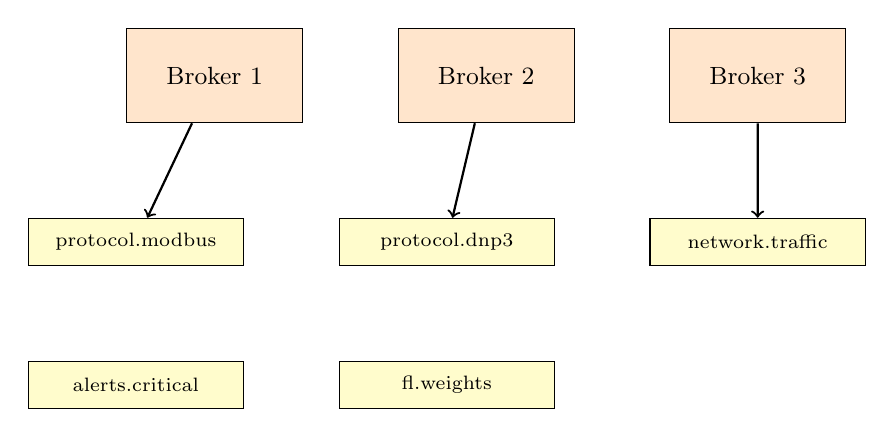
\begin{tikzpicture}[
    node distance=1.2cm,
    broker/.style={rectangle, draw, fill=orange!20, text width=2cm, align=center, minimum height=1.2cm, font=\small},
    topic/.style={rectangle, draw, fill=yellow!20, text width=2.5cm, align=center, minimum height=0.6cm, font=\scriptsize}
]

\node[broker] (b1) {Broker 1};
\node[broker, right=of b1] (b2) {Broker 2};
\node[broker, right=of b2] (b3) {Broker 3};

\node[topic, below=of b1, xshift=-1cm] (t1) {protocol.modbus};
\node[topic, right=of t1] (t2) {protocol.dnp3};
\node[topic, right=of t2] (t3) {network.traffic};
\node[topic, below=of t1] (t4) {alerts.critical};
\node[topic, right=of t4] (t5) {fl.weights};

\draw[->, thick] (b1) -- (t1);
\draw[->, thick] (b2) -- (t2);
\draw[->, thick] (b3) -- (t3);

\end{tikzpicture}
\caption{Kafka Cluster Architecture - 3 Brokers, Multiple Topics}
\end{figure}

\textbf{Purpose:} High-throughput message bus for system-wide communication

\textbf{Key Features:}
\begin{itemize}[leftmargin=1cm,itemsep=0pt]
    \item Distributed, fault-tolerant
    \item Horizontal scalability
    \item Message persistence (configurable retention)
    \item Exactly-once semantics
    \item Consumer groups for load balancing
\end{itemize}

\textbf{Topic Structure:}

\begin{table}[H]
\centering
\small
\begin{tabular}{|l|l|l|}
\hline
\textbf{Topic} & \textbf{Purpose} & \textbf{Retention} \\
\hline
protocol.modbus & Modbus messages & 7 days \\
protocol.dnp3 & DNP3 messages & 7 days \\
protocol.opcua & OPC-UA messages & 7 days \\
protocol.s7 & S7 messages & 7 days \\
network.traffic & Network flows & 3 days \\
scada.logs & SCADA events & 30 days \\
sensors.data & Sensor readings & 7 days \\
alerts.critical & Critical alerts & 90 days \\
alerts.warning & Warning alerts & 30 days \\
fl.weights & FL weight updates & 1 day \\
fl.models & FL model distributions & 7 days \\
\hline
\end{tabular}
\caption{Kafka Topics and Retention Policies}
\end{table}

\textbf{Configuration:}
\begin{lstlisting}[language=yaml]
kafka:
  brokers:
    - kafka-1:9092
    - kafka-2:9092
    - kafka-3:9092
  replication_factor: 3
  partitions: 6
  compression: snappy
  max_message_size: 10MB
\end{lstlisting}

\textbf{Performance Targets:}
\begin{itemize}[leftmargin=1cm,itemsep=0pt]
    \item Throughput: 100,000 messages/second
    \item Latency: <10ms (p99)
    \item Availability: 99.9\%
\end{itemize}

\subsection{Detection \& Analysis Layer}

\subsubsection{LSTM Autoencoder Component}

\textbf{Purpose:} Detect behavioral anomalies in time-series data

\textbf{Architecture:}

\begin{figure}[H]
\centering
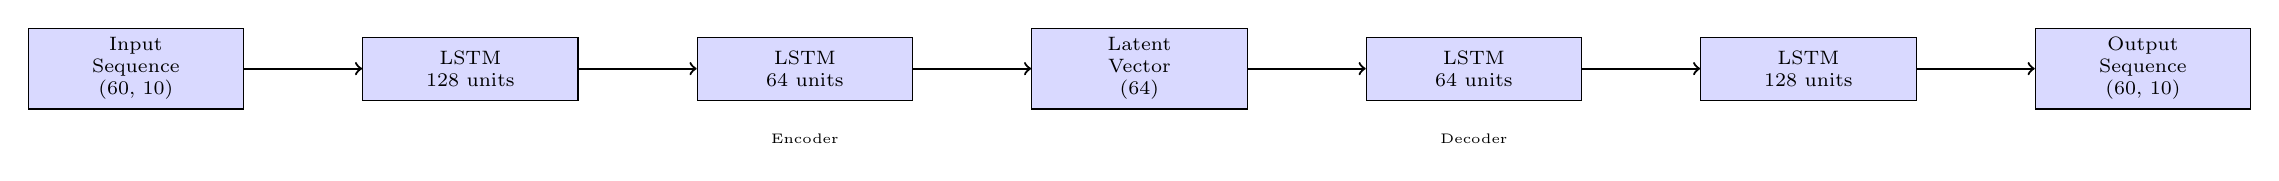
\begin{tikzpicture}[
    node distance=1.5cm,
    layer/.style={rectangle, draw, fill=blue!15, text width=2.5cm, align=center, minimum height=0.8cm, font=\scriptsize}
]

\node[layer] (input) {Input\\Sequence\\(60, 10)};
\node[layer, right=of input] (lstm1) {LSTM\\128 units};
\node[layer, right=of lstm1] (lstm2) {LSTM\\64 units};
\node[layer, right=of lstm2] (latent) {Latent\\Vector\\(64)};
\node[layer, right=of latent] (lstm3) {LSTM\\64 units};
\node[layer, right=of lstm3] (lstm4) {LSTM\\128 units};
\node[layer, right=of lstm4] (output) {Output\\Sequence\\(60, 10)};

\draw[->, thick] (input) -- (lstm1);
\draw[->, thick] (lstm1) -- (lstm2);
\draw[->, thick] (lstm2) -- (latent);
\draw[->, thick] (latent) -- (lstm3);
\draw[->, thick] (lstm3) -- (lstm4);
\draw[->, thick] (lstm4) -- (output);

\node[below=0.3cm of lstm2, font=\tiny] {Encoder};
\node[below=0.3cm of lstm3, font=\tiny] {Decoder};

\end{tikzpicture}
\caption{LSTM Autoencoder Architecture}
\end{figure}

\textbf{Responsibilities:}
\begin{itemize}[leftmargin=1cm,itemsep=0pt]
    \item Subscribe to sensor data from Kafka
    \item Create 60-second sliding windows
    \item Compute reconstruction error
    \item Flag anomalies (error > threshold)
    \item Publish alerts to Kafka
\end{itemize}

\textbf{Technology:} Python 3.9+, TensorFlow 2.x

\textbf{Hyperparameters:}
\begin{lstlisting}[language=yaml]
lstm_autoencoder:
  sequence_length: 60
  n_features: 10
  encoder_units: [128, 64]
  decoder_units: [64, 128]
  batch_size: 32
  learning_rate: 0.001
  dropout: 0.2
  threshold: 0.95  # 95th percentile
\end{lstlisting}

\textbf{Inputs:} Time-series sensor data from Kafka

\textbf{Outputs:} Anomaly alerts with reconstruction error

\textbf{Federated:} Yes - Model weights shared across facilities

\textbf{Performance:}
\begin{itemize}[leftmargin=1cm,itemsep=0pt]
    \item Inference time: <100ms per sequence
    \item Training time: ~20 minutes per epoch
    \item Memory: ~2GB
\end{itemize}

\subsubsection{Isolation Forest Component}

\textbf{Purpose:} Detect point anomalies (sudden outliers)

\textbf{Responsibilities:}
\begin{itemize}[leftmargin=1cm,itemsep=0pt]
    \item Subscribe to sensor and protocol data
    \item Compute anomaly scores
    \item Flag outliers (score > threshold)
    \item Publish alerts to Kafka
\end{itemize}

\textbf{Technology:} Python 3.9+, scikit-learn

\textbf{Hyperparameters:}
\begin{lstlisting}[language=yaml]
isolation_forest:
  n_estimators: 100
  max_samples: 256
  contamination: 0.01
  max_features: 1.0
  threshold: 0.6
\end{lstlisting}

\textbf{Federated:} Yes - Ensemble of trees shared

\textbf{Performance:}
\begin{itemize}[leftmargin=1cm,itemsep=0pt]
    \item Inference time: <10ms per sample
    \item Training time: ~5 minutes
    \item Memory: ~500MB
\end{itemize}

\subsubsection{Physics Rules Engine}

\textbf{Purpose:} Validate process physics constraints

\textbf{Responsibilities:}
\begin{itemize}[leftmargin=1cm,itemsep=0pt]
    \item Load facility-specific rules
    \item Evaluate rules against sensor data
    \item Detect violations (out of bounds, impossible rates)
    \item Publish violations to Kafka
\end{itemize}

\textbf{Technology:} Python 3.9+, custom rule engine

\textbf{Rule Types:}
\begin{itemize}[leftmargin=1cm,itemsep=0pt]
    \item \textbf{Range:} value must be in [min, max]
    \item \textbf{Rate:} change rate must be < max\_rate
    \item \textbf{Dependency:} if A then B must be true
    \item \textbf{Safety:} critical safety constraints
\end{itemize}

\textbf{Example Rules:}
\begin{lstlisting}[language=yaml]
rules:
  - name: reactor_temp_range
    type: range
    sensor: TEMP_REACTOR_01
    min: 250
    max: 350
    unit: celsius
    severity: critical
  
  - name: pressure_rate_limit
    type: rate
    sensor: PRESSURE_MAIN
    max_rate: 10
    unit: psi_per_minute
    severity: warning
  
  - name: pump_dependency
    type: dependency
    condition: VALVE_INLET == OPEN
    requirement: PUMP_01 == RUNNING
    severity: critical
\end{lstlisting}

\textbf{Federated:} No - Rules are facility-specific

\textbf{Performance:}
\begin{itemize}[leftmargin=1cm,itemsep=0pt]
    \item Evaluation time: <1ms per rule
    \item Rules per facility: 50-200
    \item Memory: <100MB
\end{itemize}

\subsubsection{Correlation Engine}

\textbf{Purpose:} Combine signals from multiple detection sources

\textbf{Architecture:}

\begin{figure}[H]
\centering
\begin{tikzpicture}[
    node distance=1cm,
    source/.style={rectangle, draw, fill=yellow!20, text width=2cm, align=center, minimum height=0.7cm, font=\scriptsize},
    engine/.style={rectangle, draw, fill=orange!20, text width=3cm, align=center, minimum height=1.5cm, font=\small},
    output/.style={rectangle, draw, fill=green!20, text width=2.5cm, align=center, minimum height=0.7cm, font=\scriptsize}
]

\node[source] (lstm) {LSTM\\Anomalies};
\node[source, below=0.5cm of lstm] (if) {Isolation\\Forest};
\node[source, below=0.5cm of if] (physics) {Physics\\Violations};
\node[source, below=0.5cm of physics] (protocol) {Protocol\\Anomalies};

\node[engine, right=2cm of if, yshift=-0.5cm] (corr) {Correlation\\Engine\\\\Temporal\\Spatial\\Severity};

\node[output, right=2cm of corr, yshift=0.5cm] (alert) {Unified\\Alert};
\node[output, below=0.5cm of alert] (incident) {Incident\\Report};

\draw[->, thick] (lstm) -- (corr);
\draw[->, thick] (if) -- (corr);
\draw[->, thick] (physics) -- (corr);
\draw[->, thick] (protocol) -- (corr);
\draw[->, thick] (corr) -- (alert);
\draw[->, thick] (corr) -- (incident);

\end{tikzpicture}
\caption{Correlation Engine - Multi-Source Fusion}
\end{figure}

\textbf{Responsibilities:}
\begin{itemize}[leftmargin=1cm,itemsep=0pt]
    \item Subscribe to all alert topics
    \item Temporal correlation (events within time window)
    \item Spatial correlation (events on related assets)
    \item Severity scoring (combine confidence scores)
    \item Generate unified threat assessments
    \item Publish to alerts.critical or alerts.warning
\end{itemize}

\textbf{Technology:} Python 3.9+, custom correlation logic

\textbf{Correlation Rules:}
\begin{lstlisting}[language=python]
# Temporal correlation
if events within 5 minutes:
    confidence *= 1.5

# Spatial correlation  
if events on same process line:
    confidence *= 1.3

# Multi-source correlation
if detected by 3+ sources:
    severity = CRITICAL
\end{lstlisting}

\textbf{Output Format:}
\begin{lstlisting}[language=json]
{
  "alert_id": "ALT-2025-10-13-001",
  "timestamp": "2025-10-13T14:23:45Z",
  "severity": "CRITICAL",
  "confidence": 0.94,
  "title": "Coordinated Attack on Reactor System",
  "affected_assets": ["PLC-REACTOR-01", "PUMP-COOLING-02"],
  "techniques": ["T0846", "T0843", "T0858"],
  "sources": ["LSTM", "IsolationForest", "PhysicsRules"],
  "timeline": [...],
  "recommended_actions": [...]
}
\end{lstlisting}

\subsubsection{Attack Prediction GNN}

\textbf{Purpose:} Predict attacker's next move using graph neural networks

\textbf{Architecture:}

\begin{figure}[H]
\centering
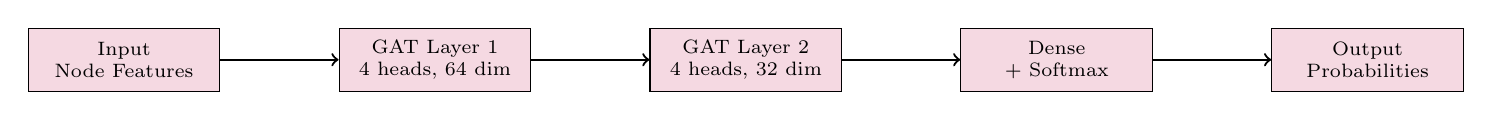
\begin{tikzpicture}[
    node distance=1.5cm,
    layer/.style={rectangle, draw, fill=purple!15, text width=2.2cm, align=center, minimum height=0.8cm, font=\scriptsize}
]

\node[layer] (input) {Input\\Node Features};
\node[layer, right=of input] (gat1) {GAT Layer 1\\4 heads, 64 dim};
\node[layer, right=of gat1] (gat2) {GAT Layer 2\\4 heads, 32 dim};
\node[layer, right=of gat2] (dense) {Dense\\+ Softmax};
\node[layer, right=of dense] (output) {Output\\Probabilities};

\draw[->, thick] (input) -- (gat1);
\draw[->, thick] (gat1) -- (gat2);
\draw[->, thick] (gat2) -- (dense);
\draw[->, thick] (dense) -- (output);

\end{tikzpicture}
\caption{Graph Attention Network for Attack Prediction}
\end{figure}

\textbf{Responsibilities:}
\begin{itemize}[leftmargin=1cm,itemsep=0pt]
    \item Load MITRE ATT\&CK graph from Neo4j
    \item Encode current attack state
    \item Predict next techniques with probabilities
    \item Publish predictions to Kafka
    \item Update graph with new attack chains
\end{itemize}

\textbf{Technology:} Python 3.9+, PyTorch, PyTorch Geometric

\textbf{Hyperparameters:}
\begin{lstlisting}[language=yaml]
gnn:
  num_techniques: 80
  hidden_dim_1: 64
  hidden_dim_2: 32
  num_heads: 4
  dropout: 0.6
  learning_rate: 0.005
  prediction_threshold: 0.5
\end{lstlisting}

\textbf{Federated:} Yes - Learns attack chains from multiple facilities

\textbf{Performance:}
\begin{itemize}[leftmargin=1cm,itemsep=0pt]
    \item Inference time: <50ms
    \item Prediction accuracy: 67\% (target)
    \item Memory: ~1GB
\end{itemize}

\textbf{Output Example:}
\begin{lstlisting}[language=json]
{
  "current_technique": "T0846",
  "predictions": [
    {"technique": "T0843", "probability": 0.67, "name": "Program Download"},
    {"technique": "T0800", "probability": 0.23, "name": "Lateral Movement"},
    {"technique": "T0858", "probability": 0.10, "name": "Change Operating Mode"}
  ],
  "target_assets": ["PLC-REACTOR-01"],
  "timeframe": "15-60 minutes"
}
\end{lstlisting}

\subsection{Federated Learning Layer}

\subsubsection{FL Architecture Overview}

\begin{figure}[H]
\centering
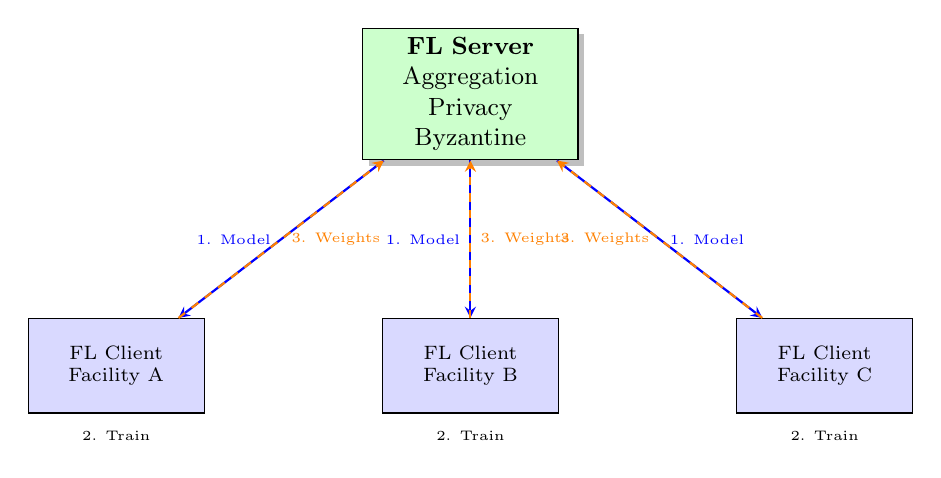
\begin{tikzpicture}[
    node distance=1.5cm,
    server/.style={rectangle, draw, fill=green!20, text width=2.5cm, align=center, minimum height=1.5cm, font=\small, drop shadow},
    client/.style={rectangle, draw, fill=blue!15, text width=2cm, align=center, minimum height=1.2cm, font=\scriptsize},
    arrow/.style={->, >=stealth, thick}
]

\node[server] (server) {\textbf{FL Server}\\Aggregation\\Privacy\\Byzantine};

\node[client, below left=2cm and 2cm of server] (c1) {FL Client\\Facility A};
\node[client, below=2cm of server] (c2) {FL Client\\Facility B};
\node[client, below right=2cm and 2cm of server] (c3) {FL Client\\Facility C};

\draw[arrow, color=blue] (server) -- node[left, font=\tiny] {1. Model} (c1);
\draw[arrow, color=blue] (server) -- node[left, font=\tiny] {1. Model} (c2);
\draw[arrow, color=blue] (server) -- node[right, font=\tiny] {1. Model} (c3);

\draw[arrow, color=orange, dashed] (c1) -- node[right, font=\tiny] {3. Weights} (server);
\draw[arrow, color=orange, dashed] (c2) -- node[right, font=\tiny] {3. Weights} (server);
\draw[arrow, color=orange, dashed] (c3) -- node[left, font=\tiny] {3. Weights} (server);

\node[below=0.1cm of c1, font=\tiny] {2. Train};
\node[below=0.1cm of c2, font=\tiny] {2. Train};
\node[below=0.1cm of c3, font=\tiny] {2. Train};

\end{tikzpicture}
\caption{Federated Learning Architecture - Server and Clients}
\end{figure}

\subsubsection{FL Client Component}

\textbf{Purpose:} Manage local training and weight transmission

\textbf{Responsibilities:}
\begin{itemize}[leftmargin=1cm,itemsep=0pt]
    \item Receive global model from FL server
    \item Train on local data (5 epochs)
    \item Compute weight updates
    \item Apply differential privacy noise
    \item Apply gradient clipping
    \item Send masked weights to server
    \item Deploy updated global model
\end{itemize}

\textbf{Technology:} Python 3.9+, Flower (flwr), TensorFlow/PyTorch

\textbf{Configuration:}
\begin{lstlisting}[language=yaml]
fl_client:
  server_address: fl-server.example.com:8080
  local_epochs: 5
  batch_size: 32
  learning_rate: 0.001
  privacy:
    epsilon: 2.0
    delta: 0.00001
    gradient_clip_norm: 1.0
  models:
    - lstm_autoencoder
    - isolation_forest
    - gnn
\end{lstlisting}

\textbf{Workflow:}
\begin{enumerate}[leftmargin=1cm,itemsep=0pt]
    \item Wait for FL round notification
    \item Download global model
    \item Load local training data
    \item Train for 5 epochs
    \item Compute weight deltas
    \item Apply gradient clipping (max\_norm=1.0)
    \item Add differential privacy noise
    \item Apply secure aggregation masks
    \item Upload to FL server
    \item Wait for next round
\end{enumerate}

\textbf{Performance:}
\begin{itemize}[leftmargin=1cm,itemsep=0pt]
    \item Training time: 20-30 minutes per round
    \item Upload size: ~10 MB
    \item Memory: 4-8 GB
\end{itemize}

\subsubsection{FL Server Component}

\textbf{Purpose:} Coordinate federated learning rounds and aggregate updates

\textbf{Responsibilities:}
\begin{itemize}[leftmargin=1cm,itemsep=0pt]
    \item Schedule FL rounds (4 per day)
    \item Distribute global model to clients
    \item Collect weight updates from clients
    \item Apply Byzantine-robust aggregation
    \item Compute new global model
    \item Distribute updated model
    \item Log metrics and monitor health
\end{itemize}

\textbf{Technology:} Python 3.9+, Flower (flwr), FastAPI

\textbf{Configuration:}
\begin{lstlisting}[language=yaml]
fl_server:
  port: 8080
  rounds_per_day: 4
  schedule: ["00:00", "06:00", "12:00", "18:00"]
  min_clients: 3
  min_fit_clients: 3
  min_available_clients: 3
  aggregation:
    method: coordinate_wise_median
    outlier_threshold: 3.0
  timeout:
    round: 40  # minutes
    client: 35  # minutes
\end{lstlisting}

\textbf{Aggregation Algorithm:}
\begin{lstlisting}[language=python]
def aggregate(weights_list):
    # Step 1: Detect outliers
    outliers = detect_outliers_zscore(weights_list, threshold=3.0)
    
    # Step 2: Filter
    clean_weights = [w for w in weights_list if w not in outliers]
    
    # Step 3: Coordinate-wise median
    aggregated = coordinate_wise_median(clean_weights)
    
    # Step 4: Log
    log_aggregation_metrics(len(clean_weights), len(outliers))
    
    return aggregated
\end{lstlisting}

\textbf{Performance:}
\begin{itemize}[leftmargin=1cm,itemsep=0pt]
    \item Aggregation time: <5 minutes
    \item Supports: 3-100 clients
    \item Memory: 8-16 GB
\end{itemize}

\subsubsection{Privacy Engine}

\textbf{Purpose:} Apply differential privacy to weight updates

\textbf{Responsibilities:}
\begin{itemize}[leftmargin=1cm,itemsep=0pt]
    \item Generate calibrated noise
    \item Add noise to gradients/weights
    \item Track privacy budget
    \item Provide privacy guarantees
\end{itemize}

\textbf{Technology:} Python 3.9+, Opacus (PyTorch), TensorFlow Privacy

\textbf{Implementation:}
\begin{lstlisting}[language=python]
from opacus import PrivacyEngine

privacy_engine = PrivacyEngine()

model, optimizer, data_loader = privacy_engine.make_private(
    module=model,
    optimizer=optimizer,
    data_loader=data_loader,
    noise_multiplier=1.1,  # Calibrated to epsilon
    max_grad_norm=1.0,
)

# Privacy budget tracking
epsilon = privacy_engine.get_epsilon(delta=1e-5)
print(f"Privacy budget: epsilon={epsilon:.2f}")
\end{lstlisting}

\textbf{Privacy Parameters:}
\begin{itemize}[leftmargin=1cm,itemsep=0pt]
    \item Epsilon (ε): 2.0 (moderate privacy)
    \item Delta (δ): 10⁻⁵ (failure probability)
    \item Noise mechanism: Gaussian
    \item Gradient clipping: L2 norm, max=1.0
\end{itemize}

\subsection{Storage Layer}

\subsubsection{Apache IoTDB - Time-Series Database}

\textbf{Purpose:} Store high-frequency sensor readings

\textbf{Schema:}
\begin{lstlisting}[language=sql]
CREATE TIMESERIES root.facility_a.reactor.temperature 
  WITH DATATYPE=FLOAT, ENCODING=GORILLA;

CREATE TIMESERIES root.facility_a.reactor.pressure 
  WITH DATATYPE=FLOAT, ENCODING=GORILLA;

CREATE TIMESERIES root.facility_a.pump.flow_rate 
  WITH DATATYPE=FLOAT, ENCODING=GORILLA;
\end{lstlisting}

\textbf{Configuration:}
\begin{lstlisting}[language=yaml]
iotdb:
  data_dir: /var/lib/iotdb/data
  wal_dir: /var/lib/iotdb/wal
  compression: SNAPPY
  retention: 7d
  replication: 3
  query_timeout: 60s
\end{lstlisting}

\textbf{Performance:}
\begin{itemize}[leftmargin=1cm,itemsep=0pt]
    \item Write throughput: 1M points/second
    \item Query latency: <100ms (p95)
    \item Compression ratio: 10:1
    \item Storage: ~100 GB per facility per month
\end{itemize}

\subsubsection{PostgreSQL - Relational Database}

\textbf{Purpose:} Store structured data (alerts, incidents, metadata)

\textbf{Schema:}
\begin{lstlisting}[language=sql]
CREATE TABLE alerts (
    alert_id VARCHAR(50) PRIMARY KEY,
    timestamp TIMESTAMP NOT NULL,
    severity VARCHAR(20) NOT NULL,
    confidence FLOAT NOT NULL,
    title TEXT NOT NULL,
    description TEXT,
    affected_assets TEXT[],
    techniques TEXT[],
    sources TEXT[],
    status VARCHAR(20) DEFAULT 'open',
    created_at TIMESTAMP DEFAULT NOW()
);

CREATE TABLE incidents (
    incident_id VARCHAR(50) PRIMARY KEY,
    start_time TIMESTAMP NOT NULL,
    end_time TIMESTAMP,
    severity VARCHAR(20) NOT NULL,
    status VARCHAR(20) DEFAULT 'investigating',
    alert_ids TEXT[],
    timeline JSONB,
    response_actions JSONB,
    created_at TIMESTAMP DEFAULT NOW()
);

CREATE INDEX idx_alerts_timestamp ON alerts(timestamp);
CREATE INDEX idx_alerts_severity ON alerts(severity);
CREATE INDEX idx_incidents_status ON incidents(status);
\end{lstlisting}

\textbf{Configuration:}
\begin{lstlisting}[language=yaml]
postgresql:
  host: postgres.example.com
  port: 5432
  database: ics_security
  max_connections: 100
  shared_buffers: 4GB
  effective_cache_size: 12GB
  backup:
    enabled: true
    schedule: "0 2 * * *"  # Daily at 2 AM
    retention: 30d
\end{lstlisting}

\subsubsection{MongoDB - Document Database}

\textbf{Purpose:} Store semi-structured data (logs, protocol messages)

\textbf{Collections:}
\begin{lstlisting}[language=javascript]
// Protocol messages
db.protocol_messages.insertOne({
  timestamp: ISODate("2025-10-13T14:23:45Z"),
  protocol: "modbus",
  source_ip: "192.168.1.10",
  function_code: 3,
  address: 1000,
  value: 42,
  metadata: {...}
});

// SCADA logs
db.scada_logs.insertOne({
  timestamp: ISODate("2025-10-13T14:23:45Z"),
  level: "INFO",
  source: "HMI-01",
  message: "Operator login: user123",
  context: {...}
});
\end{lstlisting}

\textbf{Indexes:}
\begin{lstlisting}[language=javascript]
db.protocol_messages.createIndex({timestamp: -1});
db.protocol_messages.createIndex({protocol: 1, timestamp: -1});
db.scada_logs.createIndex({timestamp: -1});
db.scada_logs.createIndex({level: 1, timestamp: -1});
\end{lstlisting}

\textbf{Configuration:}
\begin{lstlisting}[language=yaml]
mongodb:
  replicaset: rs0
  members:
    - mongodb-1:27017
    - mongodb-2:27017
    - mongodb-3:27017
  storage:
    engine: wiredTiger
    cache_size: 8GB
  retention:
    protocol_messages: 7d
    scada_logs: 30d
\end{lstlisting}

\subsubsection{Neo4j - Graph Database}

\textbf{Purpose:} Store attack graphs and MITRE ATT\&CK relationships

\textbf{Schema:}
\begin{lstlisting}[language=cypher]
// Create technique nodes
CREATE (t:Technique {
  id: 'T0846',
  name: 'Remote System Discovery',
  tactic: 'Discovery',
  description: '...'
});

// Create relationships
MATCH (a:Technique {id: 'T0846'}), (b:Technique {id: 'T0843'})
CREATE (a)-[:LEADS_TO {probability: 0.67, count: 45}]->(b);
\end{lstlisting}

\textbf{Queries:}
\begin{lstlisting}[language=cypher]
// Find most likely next techniques
MATCH (current:Technique {id: 'T0846'})-[r:LEADS_TO]->(next:Technique)
RETURN next.id, next.name, r.probability
ORDER BY r.probability DESC
LIMIT 5;

// Find attack paths
MATCH path = (start:Technique {id: 'T0846'})-[:LEADS_TO*1..5]->(end:Technique)
RETURN path
ORDER BY length(path) DESC;
\end{lstlisting}

\textbf{Configuration:}
\begin{lstlisting}[language=yaml]
neo4j:
  bolt_port: 7687
  http_port: 7474
  memory:
    heap_initial: 2G
    heap_max: 4G
    pagecache: 4G
  backup:
    enabled: true
    schedule: daily
\end{lstlisting}

\subsection{API \& Presentation Layer}

\subsubsection{REST API}

\textbf{Purpose:} Provide RESTful interface for CRUD operations

\textbf{Technology:} Python 3.9+, FastAPI

\textbf{Endpoints:}

\begin{table}[H]
\centering
\small
\begin{tabular}{|l|l|l|}
\hline
\textbf{Endpoint} & \textbf{Method} & \textbf{Description} \\
\hline
/api/v1/alerts & GET & List alerts \\
/api/v1/alerts/\{id\} & GET & Get alert details \\
/api/v1/alerts & POST & Create alert \\
/api/v1/alerts/\{id\} & PUT & Update alert \\
/api/v1/incidents & GET & List incidents \\
/api/v1/incidents/\{id\} & GET & Get incident details \\
/api/v1/predictions & GET & Get attack predictions \\
/api/v1/facilities & GET & List facilities \\
/api/v1/fl/rounds & GET & FL round history \\
/api/v1/fl/metrics & GET & FL metrics \\
/api/v1/health & GET & System health \\
\hline
\end{tabular}
\caption{REST API Endpoints}
\end{table}

\textbf{Authentication:}
\begin{lstlisting}[language=python]
from fastapi import Depends, HTTPException
from fastapi.security import HTTPBearer, HTTPAuthorizationCredentials

security = HTTPBearer()

async def verify_token(credentials: HTTPAuthorizationCredentials = Depends(security)):
    token = credentials.credentials
    if not validate_jwt(token):
        raise HTTPException(status_code=401, detail="Invalid token")
    return decode_jwt(token)
\end{lstlisting}

\textbf{Rate Limiting:}
\begin{lstlisting}[language=python]
from slowapi import Limiter
from slowapi.util import get_remote_address

limiter = Limiter(key_func=get_remote_address)

@app.get("/api/v1/alerts")
@limiter.limit("100/minute")
async def get_alerts():
    return alerts
\end{lstlisting}

\subsubsection{GraphQL API}

\textbf{Purpose:} Flexible querying for complex data relationships

\textbf{Technology:} Python 3.9+, Strawberry GraphQL

\textbf{Schema:}
\begin{lstlisting}[language=graphql]
type Alert {
  alertId: ID!
  timestamp: DateTime!
  severity: Severity!
  confidence: Float!
  title: String!
  affectedAssets: [String!]!
  techniques: [Technique!]!
  sources: [String!]!
  incident: Incident
}

type Technique {
  id: ID!
  name: String!
  tactic: String!
  nextTechniques: [TechniquePrediction!]!
}

type TechniquePrediction {
  technique: Technique!
  probability: Float!
}

type Query {
  alerts(severity: Severity, limit: Int): [Alert!]!
  alert(id: ID!): Alert
  predictions(currentTechnique: ID!): [TechniquePrediction!]!
  attackPath(start: ID!, end: ID!): [Technique!]!
}
\end{lstlisting}

\textbf{Example Query:}
\begin{lstlisting}[language=graphql]
query {
  alerts(severity: CRITICAL, limit: 10) {
    alertId
    timestamp
    title
    affectedAssets
    techniques {
      id
      name
      nextTechniques {
        technique {
          name
        }
        probability
      }
    }
  }
}
\end{lstlisting}

\subsubsection{WebSocket API}

\textbf{Purpose:} Real-time updates for dashboard

\textbf{Technology:} Python 3.9+, FastAPI WebSocket

\textbf{Implementation:}
\begin{lstlisting}[language=python]
from fastapi import WebSocket

@app.websocket("/ws/alerts")
async def websocket_alerts(websocket: WebSocket):
    await websocket.accept()
    
    # Subscribe to Kafka alerts topic
    consumer = kafka_consumer.subscribe(['alerts.critical', 'alerts.warning'])
    
    try:
        async for message in consumer:
            alert = json.loads(message.value)
            await websocket.send_json(alert)
    except WebSocketDisconnect:
        consumer.close()
\end{lstlisting}

\subsubsection{Web Dashboard}

\textbf{Purpose:} Interactive UI for operators and analysts

\textbf{Technology:} React 18+, TypeScript, Material-UI, D3.js

\textbf{Features:}
\begin{itemize}[leftmargin=1cm,itemsep=0pt]
    \item Real-time alert feed
    \item Attack graph visualization
    \item Facility status overview
    \item FL round monitoring
    \item Incident management
    \item Forensic timeline viewer
    \item Performance metrics
\end{itemize}

\textbf{Architecture:}
\begin{lstlisting}[language=typescript]
// React component structure
src/
  components/
    AlertFeed/
    AttackGraph/
    FacilityStatus/
    FLMonitor/
    IncidentManager/
    ForensicViewer/
  services/
    api.ts          // REST/GraphQL client
    websocket.ts    // WebSocket client
  store/
    alerts.ts       // Redux store
    incidents.ts
  App.tsx
\end{lstlisting}

\section{Data Flow Architecture}

\subsection{End-to-End Data Flow}

\begin{figure}[H]
\centering
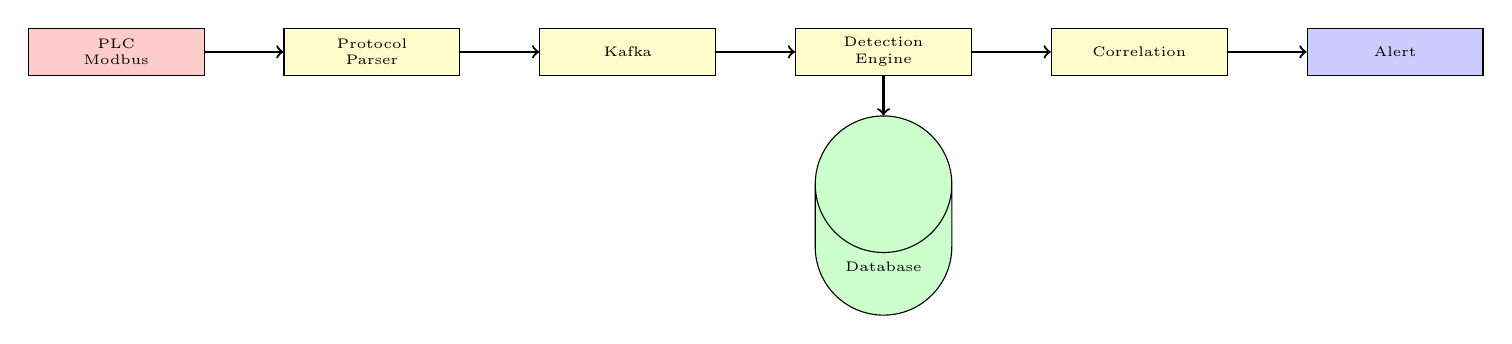
\begin{tikzpicture}[
    node distance=1cm,
    source/.style={rectangle, draw, fill=red!20, text width=2cm, align=center, minimum height=0.6cm, font=\tiny},
    process/.style={rectangle, draw, fill=yellow!20, text width=2cm, align=center, minimum height=0.6cm, font=\tiny},
    storage/.style={cylinder, draw, fill=green!20, text width=1.5cm, align=center, minimum height=0.6cm, shape border rotate=90, font=\tiny},
    output/.style={rectangle, draw, fill=blue!20, text width=2cm, align=center, minimum height=0.6cm, font=\tiny}
]

\node[source] (plc) {PLC\\Modbus};
\node[process, right=of plc] (parser) {Protocol\\Parser};
\node[process, right=of parser] (kafka) {Kafka};
\node[process, right=of kafka] (detect) {Detection\\Engine};
\node[storage, below=0.5cm of detect] (db) {Database};
\node[process, right=of detect] (corr) {Correlation};
\node[output, right=of corr] (alert) {Alert};

\draw[->, thick] (plc) -- (parser);
\draw[->, thick] (parser) -- (kafka);
\draw[->, thick] (kafka) -- (detect);
\draw[->, thick] (detect) -- (db);
\draw[->, thick] (detect) -- (corr);
\draw[->, thick] (corr) -- (alert);

\end{tikzpicture}
\caption{Simplified Data Flow - Source to Alert}
\end{figure}

\subsection{Detection Pipeline}

\textbf{Step 1: Data Ingestion}
\begin{enumerate}[leftmargin=1cm,itemsep=0pt]
    \item Protocol parsers capture industrial traffic
    \item Parse and normalize messages
    \item Publish to Kafka topics
    \item Latency: <1 second
\end{enumerate}

\textbf{Step 2: Storage}
\begin{enumerate}[leftmargin=1cm,itemsep=0pt]
    \item Consumers write to appropriate databases
    \item IoTDB: Sensor readings
    \item MongoDB: Protocol messages, logs
    \item PostgreSQL: Metadata
    \item Latency: <2 seconds
\end{enumerate}

\textbf{Step 3: Detection}
\begin{enumerate}[leftmargin=1cm,itemsep=0pt]
    \item LSTM Autoencoder analyzes sequences
    \item Isolation Forest detects outliers
    \item Physics Rules validate constraints
    \item Protocol Anomaly Detection checks messages
    \item Each publishes anomalies to Kafka
    \item Latency: <10 seconds
\end{enumerate}

\textbf{Step 4: Correlation}
\begin{enumerate}[leftmargin=1cm,itemsep=0pt]
    \item Correlation Engine subscribes to all anomaly topics
    \item Temporal correlation (5-minute window)
    \item Spatial correlation (asset relationships)
    \item Severity scoring
    \item Generate unified alert
    \item Latency: <5 seconds
\end{enumerate}

\textbf{Step 5: Prediction}
\begin{enumerate}[leftmargin=1cm,itemsep=0pt]
    \item GNN receives detected techniques
    \item Predicts next likely techniques
    \item Publishes predictions
    \item Latency: <2 seconds
\end{enumerate}

\textbf{Step 6: Alert \& Response}
\begin{enumerate}[leftmargin=1cm,itemsep=0pt]
    \item Alert published to Kafka
    \item Stored in PostgreSQL
    \item Pushed to dashboard via WebSocket
    \item Notifications sent (email, SMS, SIEM)
    \item Latency: <5 seconds
\end{enumerate}

\textbf{Total End-to-End Latency: <30 seconds}

\subsection{Federated Learning Data Flow}

\textbf{Round Workflow:}

\begin{enumerate}[leftmargin=1cm,itemsep=0pt]
    \item \textbf{00:00 - Round Start}
    \begin{itemize}[leftmargin=0.5cm,itemsep=0pt]
        \item FL Server broadcasts round start
        \item Sends current global model to clients
    \end{itemize}
    
    \item \textbf{00:05 - Local Training}
    \begin{itemize}[leftmargin=0.5cm,itemsep=0pt]
        \item Each facility loads local data
        \item Trains model for 5 epochs
        \item Computes weight updates
    \end{itemize}
    
    \item \textbf{00:30 - Privacy Protection}
    \begin{itemize}[leftmargin=0.5cm,itemsep=0pt]
        \item Apply gradient clipping (max\_norm=1.0)
        \item Add differential privacy noise (ε=2.0)
        \item Apply secure aggregation masks
    \end{itemize}
    
    \item \textbf{00:35 - Upload}
    \begin{itemize}[leftmargin=0.5cm,itemsep=0pt]
        \item Facilities upload masked weights (~10 MB)
        \item Server collects updates
    \end{itemize}
    
    \item \textbf{00:40 - Aggregation}
    \begin{itemize}[leftmargin=0.5cm,itemsep=0pt]
        \item Detect outliers (Byzantine-robust)
        \item Compute coordinate-wise median
        \item Create new global model
    \end{itemize}
    
    \item \textbf{00:45 - Distribution}
    \begin{itemize}[leftmargin=0.5cm,itemsep=0pt]
        \item Distribute updated model to all facilities
        \item Facilities deploy new model
    \end{itemize}
    
    \item \textbf{06:00 - Next Round}
\end{enumerate}

\section{Security Architecture}

\subsection{Defense in Depth}

\begin{figure}[H]
\centering
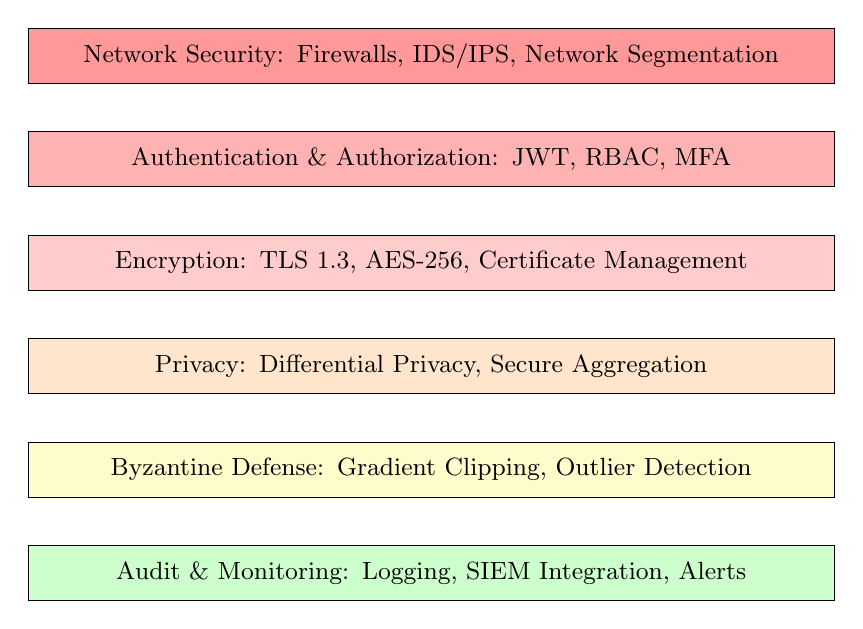
\begin{tikzpicture}[
    node distance=0.6cm,
    layer/.style={rectangle, draw, fill=red!20, text width=10cm, align=center, minimum height=0.7cm, font=\small}
]

\node[layer, fill=red!40] (net) {Network Security: Firewalls, IDS/IPS, Network Segmentation};
\node[layer, below=of net, fill=red!30] (auth) {Authentication \& Authorization: JWT, RBAC, MFA};
\node[layer, below=of auth, fill=red!20] (encrypt) {Encryption: TLS 1.3, AES-256, Certificate Management};
\node[layer, below=of encrypt, fill=orange!20] (privacy) {Privacy: Differential Privacy, Secure Aggregation};
\node[layer, below=of privacy, fill=yellow!20] (byzantine) {Byzantine Defense: Gradient Clipping, Outlier Detection};
\node[layer, below=of byzantine, fill=green!20] (audit) {Audit \& Monitoring: Logging, SIEM Integration, Alerts};

\end{tikzpicture}
\caption{Security Layers - Defense in Depth}
\end{figure}

\subsection{Authentication \& Authorization}

\subsubsection{Authentication}

\textbf{JWT-Based Authentication:}
\begin{lstlisting}[language=python]
from jose import jwt
from datetime import datetime, timedelta

def create_access_token(user_id: str, roles: List[str]):
    payload = {
        "sub": user_id,
        "roles": roles,
        "exp": datetime.utcnow() + timedelta(hours=1),
        "iat": datetime.utcnow()
    }
    return jwt.encode(payload, SECRET_KEY, algorithm="HS256")
\end{lstlisting}

\textbf{Multi-Factor Authentication (MFA):}
\begin{itemize}[leftmargin=1cm,itemsep=0pt]
    \item TOTP (Time-based One-Time Password)
    \item SMS backup codes
    \item Hardware tokens (YubiKey)
\end{itemize}

\subsubsection{Authorization}

\textbf{Role-Based Access Control (RBAC):}

\begin{table}[H]
\centering
\small
\begin{tabular}{|l|l|}
\hline
\textbf{Role} & \textbf{Permissions} \\
\hline
Admin & Full system access, user management \\
Analyst & View alerts, incidents, create reports \\
Operator & View alerts, acknowledge, basic actions \\
Viewer & Read-only access to dashboards \\
FL\_Participant & Participate in federated learning \\
\hline
\end{tabular}
\caption{RBAC Roles and Permissions}
\end{table}

\textbf{Implementation:}
\begin{lstlisting}[language=python]
from fastapi import Depends

def require_role(required_role: str):
    def role_checker(user = Depends(get_current_user)):
        if required_role not in user.roles:
            raise HTTPException(status_code=403, detail="Insufficient permissions")
        return user
    return role_checker

@app.get("/api/v1/admin/users")
async def get_users(user = Depends(require_role("Admin"))):
    return users
\end{lstlisting}

\subsection{Network Security}

\subsubsection{Network Segmentation}

\begin{figure}[H]
\centering
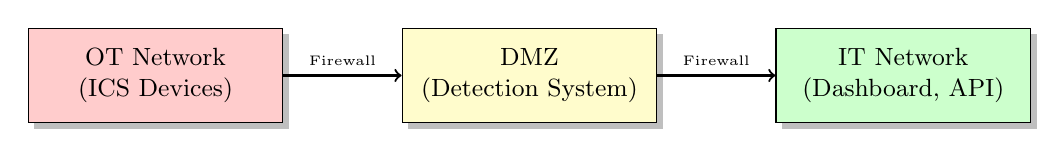
\begin{tikzpicture}[
    node distance=1.5cm,
    zone/.style={rectangle, draw, fill=blue!15, text width=3cm, align=center, minimum height=1.2cm, font=\small, drop shadow}
]

\node[zone, fill=red!20] (ot) {OT Network\\(ICS Devices)};
\node[zone, right=of ot, fill=yellow!20] (dmz) {DMZ\\(Detection System)};
\node[zone, right=of dmz, fill=green!20] (it) {IT Network\\(Dashboard, API)};

\draw[->, thick] (ot) -- node[above, font=\tiny] {Firewall} (dmz);
\draw[->, thick] (dmz) -- node[above, font=\tiny] {Firewall} (it);

\end{tikzpicture}
\caption{Network Segmentation - Three Zones}
\end{figure}

\textbf{Firewall Rules:}
\begin{itemize}[leftmargin=1cm,itemsep=0pt]
    \item OT → DMZ: Allow Modbus (502), DNP3 (20000), OPC-UA (4840)
    \item DMZ → IT: Allow HTTPS (443), WebSocket (8080)
    \item IT → DMZ: Allow API calls (8000)
    \item Deny all other traffic
\end{itemize}

\subsubsection{Encryption}

\textbf{Data in Transit:}
\begin{itemize}[leftmargin=1cm,itemsep=0pt]
    \item TLS 1.3 for all external communication
    \item Certificate-based mutual authentication
    \item Perfect Forward Secrecy (PFS)
    \item Cipher suites: TLS\_AES\_256\_GCM\_SHA384
\end{itemize}

\textbf{Data at Rest:}
\begin{itemize}[leftmargin=1cm,itemsep=0pt]
    \item AES-256 encryption for databases
    \item Encrypted backups
    \item Key rotation every 90 days
    \item Hardware Security Module (HSM) for key storage
\end{itemize}

\textbf{FL Communication:}
\begin{lstlisting}[language=python]
import ssl

ssl_context = ssl.create_default_context(ssl.Purpose.CLIENT_AUTH)
ssl_context.load_cert_chain(certfile="server.crt", keyfile="server.key")
ssl_context.load_verify_locations(cafile="ca.crt")
ssl_context.verify_mode = ssl.CERT_REQUIRED

# Use with gRPC or HTTPS
\end{lstlisting}

\subsection{Privacy Protection}

\subsubsection{Multi-Layer Privacy}

\textbf{Layer 1: Data Isolation}
\begin{itemize}[leftmargin=1cm,itemsep=0pt]
    \item Raw data never leaves facility
    \item Only model weights transmitted
    \item Local storage and processing
\end{itemize}

\textbf{Layer 2: Differential Privacy}
\begin{itemize}[leftmargin=1cm,itemsep=0pt]
    \item Calibrated noise added to weights
    \item (ε=2.0, δ=10⁻⁵) guarantees
    \item Privacy budget tracking
\end{itemize}

\textbf{Layer 3: Secure Aggregation}
\begin{itemize}[leftmargin=1cm,itemsep=0pt]
    \item Server cannot see individual updates
    \item Pairwise masking
    \item Cryptographic protection
\end{itemize}

\textbf{Layer 4: Gradient Clipping}
\begin{itemize}[leftmargin=1cm,itemsep=0pt]
    \item Limits update magnitude
    \item max\_norm = 1.0
    \item Prevents information leakage
\end{itemize}

\textbf{Layer 5: Byzantine-Robust Aggregation}
\begin{itemize}[leftmargin=1cm,itemsep=0pt]
    \item Detects malicious updates
    \item Coordinate-wise median
    \item Outlier exclusion
\end{itemize}

\subsection{Audit \& Compliance}

\subsubsection{Audit Logging}

\textbf{Logged Events:}
\begin{itemize}[leftmargin=1cm,itemsep=0pt]
    \item User authentication (success/failure)
    \item Authorization decisions
    \item Data access (queries, exports)
    \item Configuration changes
    \item Alert creation and acknowledgment
    \item FL round participation
    \item System errors and exceptions
\end{itemize}

\textbf{Log Format:}
\begin{lstlisting}[language=json]
{
  "timestamp": "2025-10-13T14:23:45Z",
  "event_type": "authentication",
  "user_id": "user123",
  "action": "login",
  "result": "success",
  "ip_address": "192.168.1.100",
  "user_agent": "Mozilla/5.0...",
  "metadata": {...}
}
\end{lstlisting}

\textbf{Log Storage:}
\begin{itemize}[leftmargin=1cm,itemsep=0pt]
    \item Centralized logging (ELK Stack or Splunk)
    \item Immutable audit trail
    \item Retention: 1 year minimum
    \item Encrypted storage
    \item Regular integrity checks
\end{itemize}

\subsubsection{Compliance}

\textbf{NERC CIP (North American Electric Reliability Corporation):}
\begin{itemize}[leftmargin=1cm,itemsep=0pt]
    \item CIP-005: Electronic Security Perimeter
    \item CIP-007: System Security Management
    \item CIP-010: Configuration Change Management
    \item CIP-011: Information Protection
\end{itemize}

\textbf{IEC 62443 (Industrial Automation and Control Systems Security):}
\begin{itemize}[leftmargin=1cm,itemsep=0pt]
    \item Network segmentation
    \item Access control
    \item Data integrity
    \item Availability requirements
\end{itemize}

\textbf{GDPR (General Data Protection Regulation):}
\begin{itemize}[leftmargin=1cm,itemsep=0pt]
    \item Data minimization (only weights shared)
    \item Privacy by design
    \item Right to erasure
    \item Data protection impact assessment
\end{itemize}

\section{Deployment Architecture}

\subsection{Development Environment}

\textbf{Docker Compose Setup:}
\begin{lstlisting}[language=yaml]
version: '3.8'

services:
  kafka:
    image: confluentinc/cp-kafka:7.4.0
    ports:
      - "9092:9092"
  
  iotdb:
    image: apache/iotdb:1.2.0
    ports:
      - "6667:6667"
  
  postgres:
    image: postgres:15
    environment:
      POSTGRES_DB: ics_security
      POSTGRES_PASSWORD: ${DB_PASSWORD}
  
  mongodb:
    image: mongo:6.0
    ports:
      - "27017:27017"
  
  neo4j:
    image: neo4j:5.11
    ports:
      - "7474:7474"
      - "7687:7687"
  
  detection-engine:
    build: ./detection
    depends_on:
      - kafka
      - iotdb
  
  fl-server:
    build: ./fl-server
    ports:
      - "8080:8080"
  
  api:
    build: ./api
    ports:
      - "8000:8000"
    depends_on:
      - postgres
      - mongodb
  
  dashboard:
    build: ./dashboard
    ports:
      - "3000:3000"
\end{lstlisting}

\subsection{Production Environment - Kubernetes}

\textbf{Cluster Architecture:}

\begin{figure}[H]
\centering
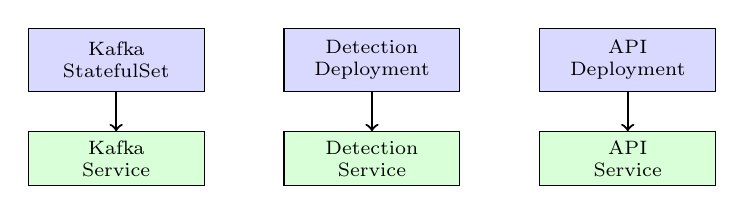
\begin{tikzpicture}[
    node distance=1cm,
    pod/.style={rectangle, draw, fill=blue!15, text width=2cm, align=center, minimum height=0.8cm, font=\scriptsize},
    service/.style={rectangle, draw, fill=green!15, text width=2cm, align=center, minimum height=0.6cm, font=\scriptsize}
]

\node[pod] (kafka) {Kafka\\StatefulSet};
\node[pod, right=of kafka] (detect) {Detection\\Deployment};
\node[pod, right=of detect] (api) {API\\Deployment};

\node[service, below=0.5cm of kafka] (kafka-svc) {Kafka\\Service};
\node[service, below=0.5cm of detect] (detect-svc) {Detection\\Service};
\node[service, below=0.5cm of api] (api-svc) {API\\Service};

\draw[->, thick] (kafka) -- (kafka-svc);
\draw[->, thick] (detect) -- (detect-svc);
\draw[->, thick] (api) -- (api-svc);

\end{tikzpicture}
\caption{Kubernetes Deployment - Pods and Services}
\end{figure}

\textbf{Deployment Manifests:}
\begin{lstlisting}[language=yaml]
# Detection Engine Deployment
apiVersion: apps/v1
kind: Deployment
metadata:
  name: detection-engine
spec:
  replicas: 3
  selector:
    matchLabels:
      app: detection-engine
  template:
    metadata:
      labels:
        app: detection-engine
    spec:
      containers:
      - name: detection
        image: ics-detection:1.0
        resources:
          requests:
            memory: "4Gi"
            cpu: "2"
          limits:
            memory: "8Gi"
            cpu: "4"
        env:
        - name: KAFKA_BROKERS
          value: "kafka-0.kafka:9092,kafka-1.kafka:9092"
        - name: IOTDB_HOST
          value: "iotdb-service"
---
# Horizontal Pod Autoscaler
apiVersion: autoscaling/v2
kind: HorizontalPodAutoscaler
metadata:
  name: detection-engine-hpa
spec:
  scaleTargetRef:
    apiVersion: apps/v1
    kind: Deployment
    name: detection-engine
  minReplicas: 3
  maxReplicas: 10
  metrics:
  - type: Resource
    resource:
      name: cpu
      target:
        type: Utilization
        averageUtilization: 70
\end{lstlisting}

\subsection{Cloud Deployment Options}

\subsubsection{AWS Architecture}

\textbf{Services:}
\begin{itemize}[leftmargin=1cm,itemsep=0pt]
    \item \textbf{EKS:} Kubernetes cluster
    \item \textbf{MSK:} Managed Kafka
    \item \textbf{RDS:} PostgreSQL
    \item \textbf{DocumentDB:} MongoDB-compatible
    \item \textbf{Neptune:} Graph database
    \item \textbf{S3:} Object storage for backups
    \item \textbf{CloudWatch:} Monitoring and logging
    \item \textbf{ALB:} Application Load Balancer
    \item \textbf{Route53:} DNS management
\end{itemize}

\subsubsection{Azure Architecture}

\textbf{Services:}
\begin{itemize}[leftmargin=1cm,itemsep=0pt]
    \item \textbf{AKS:} Kubernetes cluster
    \item \textbf{Event Hubs:} Kafka-compatible messaging
    \item \textbf{Azure Database for PostgreSQL:} Managed PostgreSQL
    \item \textbf{Cosmos DB:} Multi-model database
    \item \textbf{Blob Storage:} Object storage
    \item \textbf{Azure Monitor:} Monitoring and logging
    \item \textbf{Application Gateway:} Load balancer
    \item \textbf{Azure DNS:} DNS management
\end{itemize}

\subsubsection{On-Premise Deployment}

\textbf{Hardware Requirements:}

\begin{table}[H]
\centering
\small
\begin{tabular}{|l|l|l|l|}
\hline
\textbf{Component} & \textbf{CPU} & \textbf{RAM} & \textbf{Storage} \\
\hline
Kafka Cluster (3 nodes) & 8 cores & 32 GB & 2 TB SSD \\
Detection Engine (3 nodes) & 8 cores & 32 GB & 500 GB \\
Database Cluster (3 nodes) & 16 cores & 64 GB & 4 TB SSD \\
FL Server & 16 cores & 64 GB & 1 TB \\
API/Dashboard (2 nodes) & 8 cores & 16 GB & 500 GB \\
\hline
\textbf{Total} & \textbf{120 cores} & \textbf{368 GB} & \textbf{15.5 TB} \\
\hline
\end{tabular}
\caption{On-Premise Hardware Requirements}
\end{table}

\section{Scalability \& Performance}

\subsection{Horizontal Scaling}

\textbf{Stateless Components (Easy to Scale):}
\begin{itemize}[leftmargin=1cm,itemsep=0pt]
    \item Detection engines
    \item API servers
    \item Dashboard servers
    \item Protocol parsers
\end{itemize}

\textbf{Stateful Components (Require Coordination):}
\begin{itemize}[leftmargin=1cm,itemsep=0pt]
    \item Kafka brokers (add partitions)
    \item Database clusters (sharding)
    \item FL server (single instance, but can handle 100+ clients)
\end{itemize}

\subsection{Performance Targets}

\begin{table}[H]
\centering
\small
\begin{tabular}{|l|l|l|}
\hline
\textbf{Metric} & \textbf{Target} & \textbf{Measurement} \\
\hline
Detection Latency & <30 seconds & Event to alert \\
API Response Time & <100ms & p95 \\
Dashboard Load Time & <2 seconds & Initial load \\
Kafka Throughput & 100K msg/s & Messages per second \\
Database Write & 10K writes/s & Inserts per second \\
Database Query & <100ms & p95 query time \\
FL Round Time & <40 minutes & Complete round \\
System Availability & 99.9\% & Uptime \\
\hline
\end{tabular}
\caption{Performance Targets}
\end{table}

\subsection{Bottleneck Mitigation}

\textbf{Kafka:}
\begin{itemize}[leftmargin=1cm,itemsep=0pt]
    \item Increase partitions for parallel processing
    \item Add brokers for higher throughput
    \item Tune retention policies
    \item Use compression (snappy)
\end{itemize}

\textbf{Databases:}
\begin{itemize}[leftmargin=1cm,itemsep=0pt]
    \item Read replicas for query load
    \item Sharding for write load
    \item Indexing optimization
    \item Query caching (Redis)
\end{itemize}

\textbf{Detection Engines:}
\begin{itemize}[leftmargin=1cm,itemsep=0pt]
    \item Horizontal scaling (add more instances)
    \item GPU acceleration for LSTM/GNN
    \item Model optimization (quantization, pruning)
    \item Batch processing
\end{itemize}

\subsection{Caching Strategy}

\textbf{Redis Cache:}
\begin{lstlisting}[language=python]
import redis

cache = redis.Redis(host='redis', port=6379, db=0)

# Cache alert data
def get_alert(alert_id: str):
    # Try cache first
    cached = cache.get(f"alert:{alert_id}")
    if cached:
        return json.loads(cached)
    
    # Query database
    alert = db.query_alert(alert_id)
    
    # Cache for 5 minutes
    cache.setex(f"alert:{alert_id}", 300, json.dumps(alert))
    
    return alert
\end{lstlisting}

\textbf{Cache Layers:}
\begin{itemize}[leftmargin=1cm,itemsep=0pt]
    \item \textbf{L1:} In-memory (application)
    \item \textbf{L2:} Redis (distributed)
    \item \textbf{L3:} Database query cache
\end{itemize}

\section{Monitoring \& Observability}

\subsection{Metrics Collection}

\textbf{Prometheus Metrics:}
\begin{lstlisting}[language=python]
from prometheus_client import Counter, Histogram, Gauge

# Counters
alerts_total = Counter('alerts_total', 'Total alerts', ['severity'])
fl_rounds_total = Counter('fl_rounds_total', 'Total FL rounds')

# Histograms
detection_latency = Histogram('detection_latency_seconds', 
                              'Detection latency')
api_request_duration = Histogram('api_request_duration_seconds',
                                 'API request duration', ['endpoint'])

# Gauges
active_facilities = Gauge('active_facilities', 'Active facilities')
kafka_lag = Gauge('kafka_consumer_lag', 'Kafka consumer lag', ['topic'])

# Usage
alerts_total.labels(severity='critical').inc()
detection_latency.observe(0.025)  # 25ms
\end{lstlisting}

\textbf{Key Metrics:}
\begin{itemize}[leftmargin=1cm,itemsep=0pt]
    \item Detection latency (p50, p95, p99)
    \item Alert rate (per minute)
    \item False positive rate
    \item FL round completion time
    \item FL participant count
    \item Model accuracy
    \item API response time
    \item Database query time
    \item Kafka consumer lag
    \item System resource usage (CPU, memory, disk)
\end{itemize}

\subsection{Logging Strategy}

\textbf{Structured Logging:}
\begin{lstlisting}[language=python]
import structlog

logger = structlog.get_logger()

logger.info("alert_created",
    alert_id="ALT-2025-10-13-001",
    severity="critical",
    confidence=0.94,
    techniques=["T0846", "T0843"],
    facility="facility_a"
)
\end{lstlisting}

\textbf{Log Levels:}
\begin{itemize}[leftmargin=1cm,itemsep=0pt]
    \item \textbf{DEBUG:} Detailed diagnostic information
    \item \textbf{INFO:} General informational messages
    \item \textbf{WARNING:} Warning messages (potential issues)
    \item \textbf{ERROR:} Error messages (failures)
    \item \textbf{CRITICAL:} Critical errors (system failure)
\end{itemize}

\subsection{Alerting Rules}

\textbf{Prometheus Alerting:}
\begin{lstlisting}[language=yaml]
groups:
- name: ics_security
  rules:
  - alert: HighDetectionLatency
    expr: detection_latency_seconds{quantile="0.95"} > 30
    for: 5m
    labels:
      severity: warning
    annotations:
      summary: "Detection latency exceeds 30 seconds"
  
  - alert: FLRoundFailed
    expr: increase(fl_rounds_failed_total[1h]) > 0
    labels:
      severity: critical
    annotations:
      summary: "FL round failed"
  
  - alert: LowFLParticipation
    expr: active_facilities < 3
    for: 10m
    labels:
      severity: warning
    annotations:
      summary: "Less than 3 facilities participating in FL"
  
  - alert: HighFalsePositiveRate
    expr: false_positive_rate > 0.10
    for: 15m
    labels:
      severity: warning
    annotations:
      summary: "False positive rate exceeds 10%"
\end{lstlisting}

\subsection{Dashboards}

\textbf{Grafana Dashboards:}
\begin{itemize}[leftmargin=1cm,itemsep=0pt]
    \item \textbf{System Overview:} High-level metrics, health status
    \item \textbf{Detection Performance:} Latency, accuracy, false positives
    \item \textbf{FL Monitoring:} Round status, participants, model accuracy
    \item \textbf{Infrastructure:} CPU, memory, disk, network
    \item \textbf{Security:} Authentication failures, suspicious activity
    \item \textbf{Business Metrics:} Alerts per day, incident resolution time
\end{itemize}

\section{Technology Stack Summary}

\subsection{Backend}

\begin{table}[H]
\centering
\small
\begin{tabular}{|l|l|l|}
\hline
\textbf{Component} & \textbf{Technology} & \textbf{Version} \\
\hline
Language & Python & 3.9+ \\
Web Framework & FastAPI & 0.104+ \\
ML Framework & TensorFlow / PyTorch & 2.14+ / 2.1+ \\
FL Framework & Flower (flwr) & 1.5+ \\
Privacy & Opacus & 1.4+ \\
GNN & PyTorch Geometric & 2.4+ \\
\hline
\end{tabular}
\caption{Backend Technology Stack}
\end{table}

\subsection{Protocols \& Messaging}

\begin{table}[H]
\centering
\small
\begin{tabular}{|l|l|l|}
\hline
\textbf{Component} & \textbf{Technology} & \textbf{Version} \\
\hline
Modbus & pyModbus & 3.5+ \\
DNP3 & dnp3-python & 0.2+ \\
OPC-UA & opcua & 0.98+ \\
S7 & python-snap7 & 1.3+ \\
Network Capture & scapy & 2.5+ \\
Message Bus & Apache Kafka & 3.5+ \\
\hline
\end{tabular}
\caption{Protocols \& Messaging Stack}
\end{table}

\subsection{Storage}

\begin{table}[H]
\centering
\small
\begin{tabular}{|l|l|l|}
\hline
\textbf{Component} & \textbf{Technology} & \textbf{Version} \\
\hline
Time-Series DB & Apache IoTDB & 1.2+ \\
Relational DB & PostgreSQL & 15+ \\
Document DB & MongoDB & 6.0+ \\
Graph DB & Neo4j & 5.11+ \\
Cache & Redis & 7.2+ \\
\hline
\end{tabular}
\caption{Storage Technology Stack}
\end{table}

\subsection{Frontend}

\begin{table}[H]
\centering
\small
\begin{tabular}{|l|l|l|}
\hline
\textbf{Component} & \textbf{Technology} & \textbf{Version} \\
\hline
Framework & React & 18+ \\
Language & TypeScript & 5.0+ \\
UI Library & Material-UI & 5.14+ \\
Visualization & D3.js & 7.8+ \\
State Management & Redux Toolkit & 1.9+ \\
API Client & Axios & 1.5+ \\
\hline
\end{tabular}
\caption{Frontend Technology Stack}
\end{table}

\subsection{DevOps \& Infrastructure}

\begin{table}[H]
\centering
\small
\begin{tabular}{|l|l|l|}
\hline
\textbf{Component} & \textbf{Technology} & \textbf{Version} \\
\hline
Containerization & Docker & 24+ \\
Orchestration & Kubernetes & 1.28+ \\
CI/CD & GitHub Actions & - \\
Monitoring & Prometheus & 2.47+ \\
Visualization & Grafana & 10.1+ \\
Logging & ELK Stack & 8.10+ \\
\hline
\end{tabular}
\caption{DevOps Technology Stack}
\end{table}

\section{Conclusion}

This architecture document provides a comprehensive blueprint for implementing the Federated ICS Threat Correlation Engine. The system is designed with the following key characteristics:

\textbf{Scalable:} Horizontal scaling for all stateless components, supporting 10-1000+ facilities.

\textbf{Secure:} Multi-layer security with defense in depth, encryption, authentication, and privacy protection.

\textbf{Performant:} <30 second detection latency, >95\% accuracy, <5\% false positives.

\textbf{Privacy-Preserving:} Differential privacy, secure aggregation, and Byzantine-robust defenses.

\textbf{Observable:} Comprehensive monitoring, logging, and alerting for production operations.

\textbf{Maintainable:} Modular architecture with clear component boundaries and well-defined interfaces.

The architecture supports incremental deployment from development (Docker Compose) to production (Kubernetes) to enterprise scale (cloud-native), enabling organizations to start small and scale as needed.

\end{document}
